\documentclass{article}
\usepackage{amsmath}
\usepackage{enumerate}
\usepackage{listings}
\usepackage{moreverb}
\usepackage[margin=1in]{geometry}
\usepackage{graphicx}
\usepackage{dsfont}
\title{STA 360: Lab 10}
\author{Michael Lin}

\begin{document}
\maketitle

\begin{enumerate}
\item From last week:

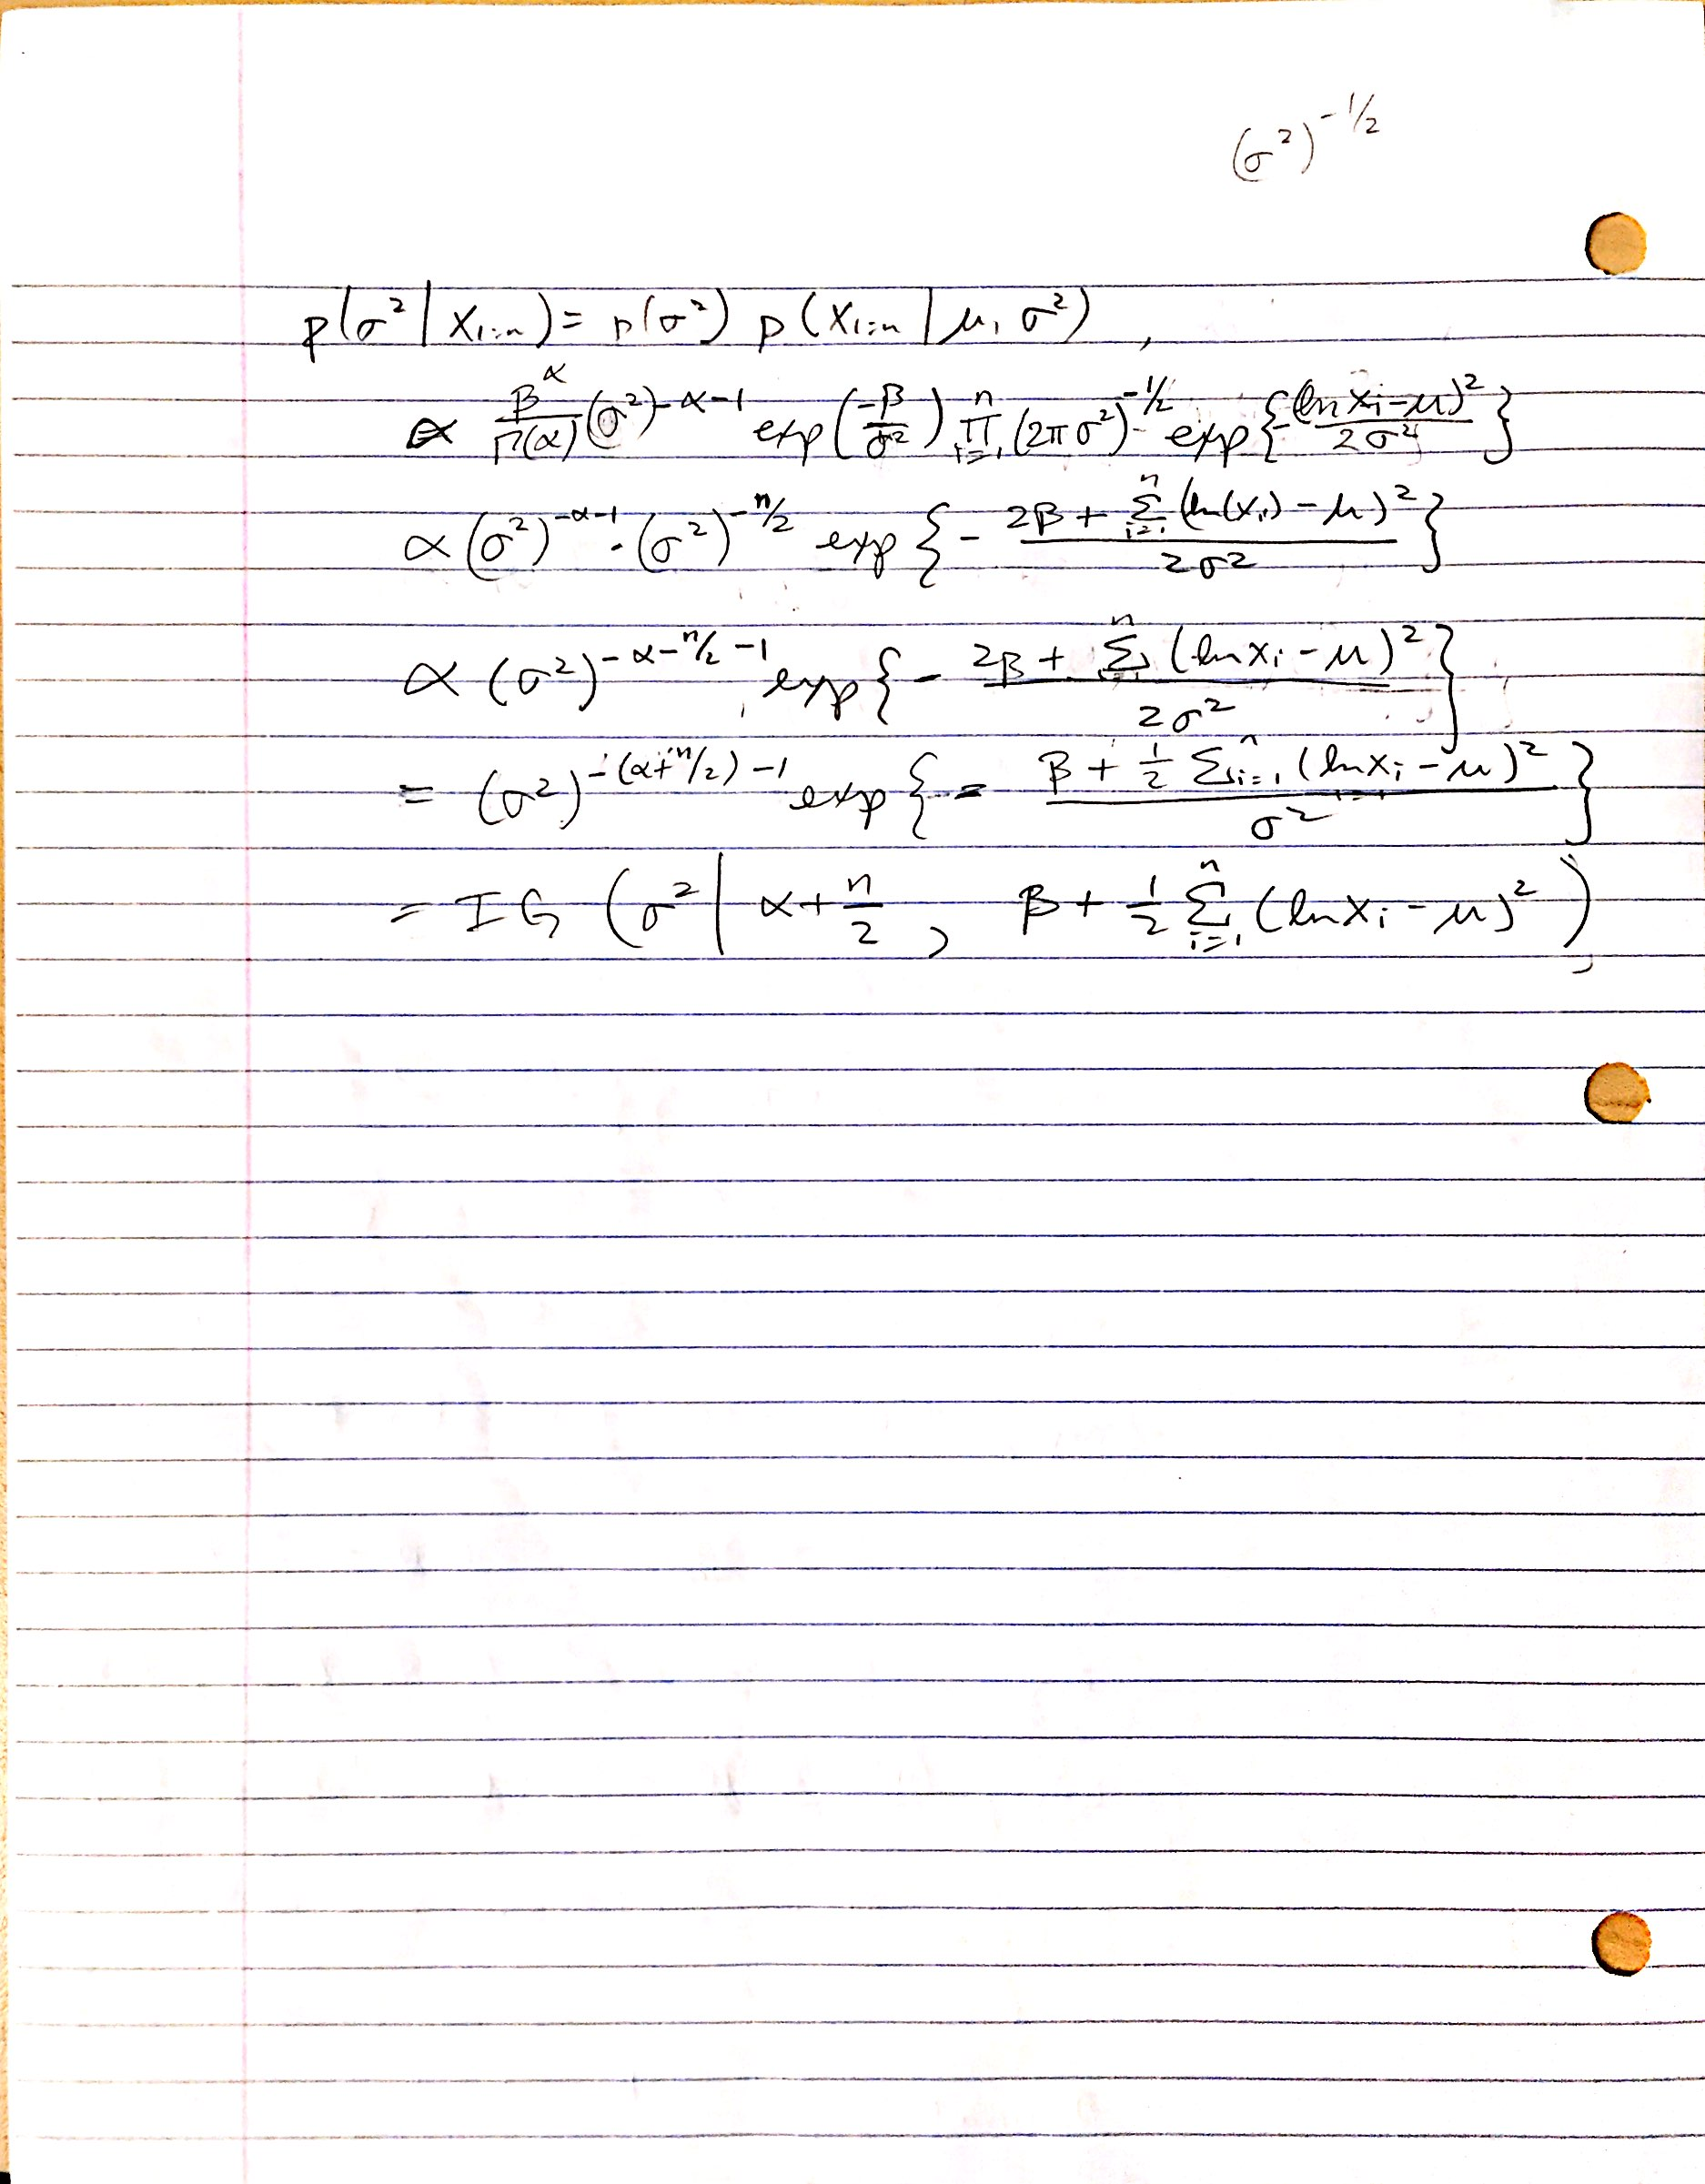
\includegraphics[scale=0.2]{page4.jpg} \\

\pagebreak
The model for this week:

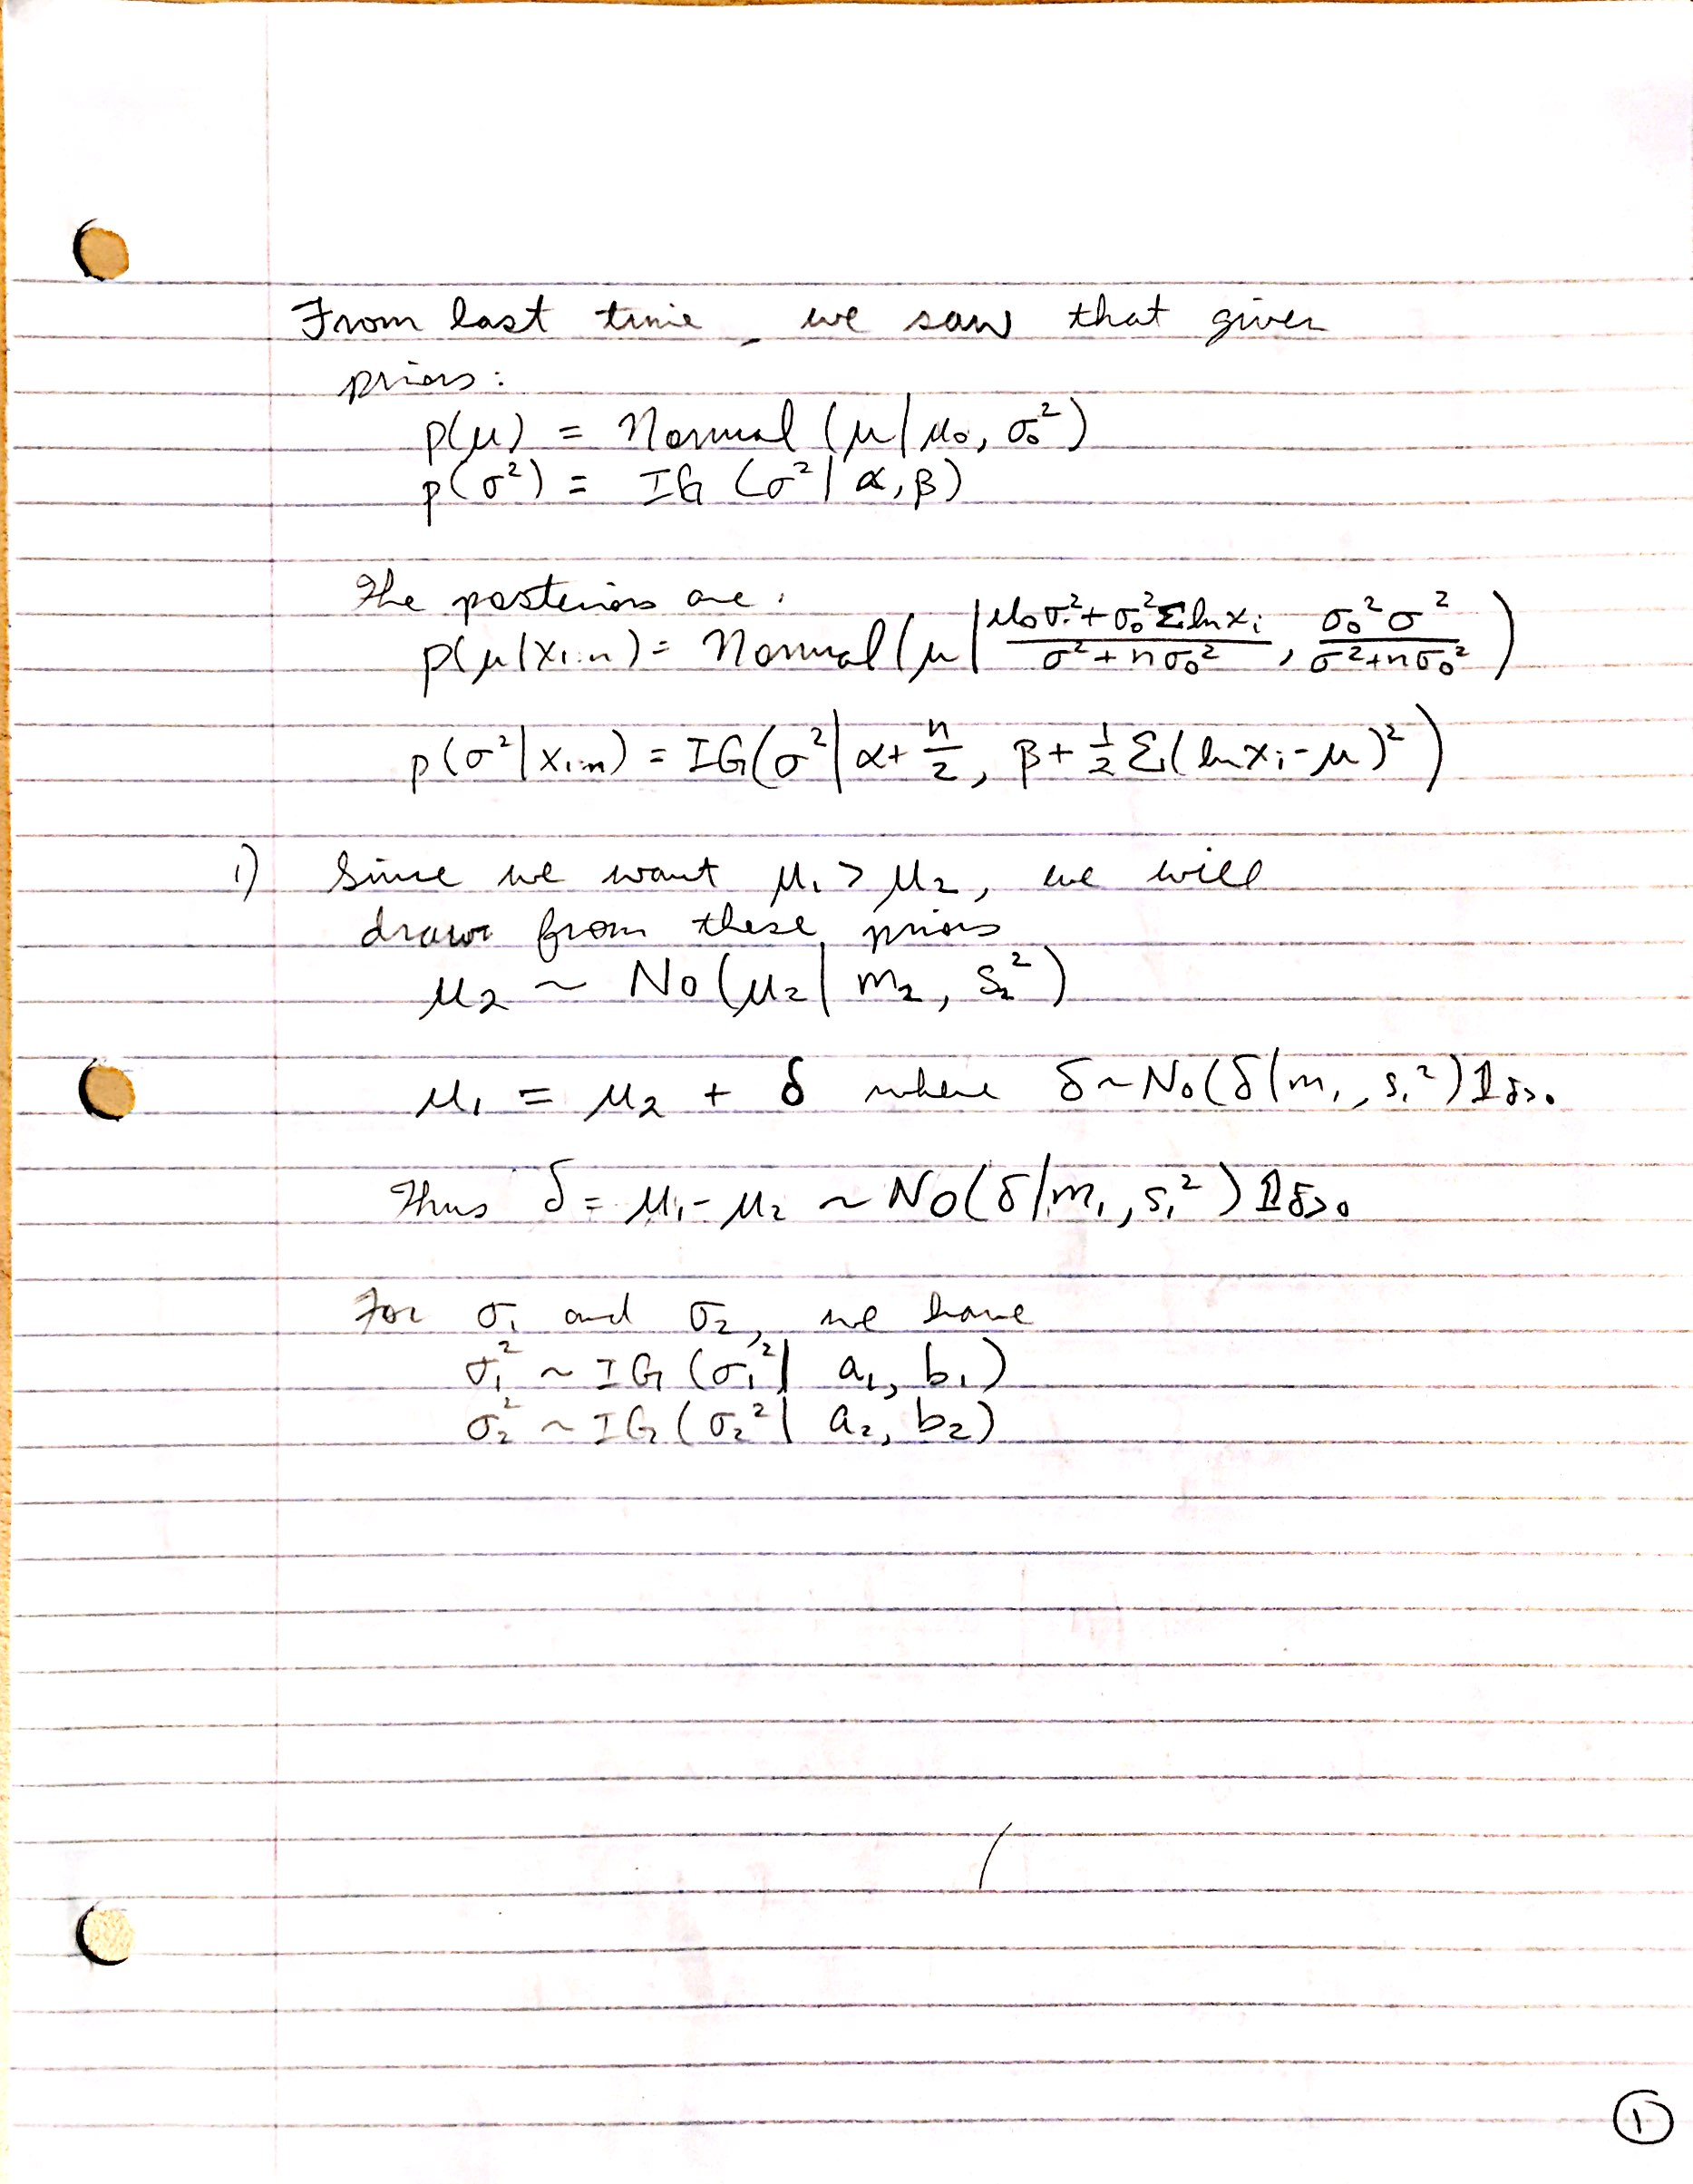
\includegraphics[scale=0.23]{page1.jpg} \\
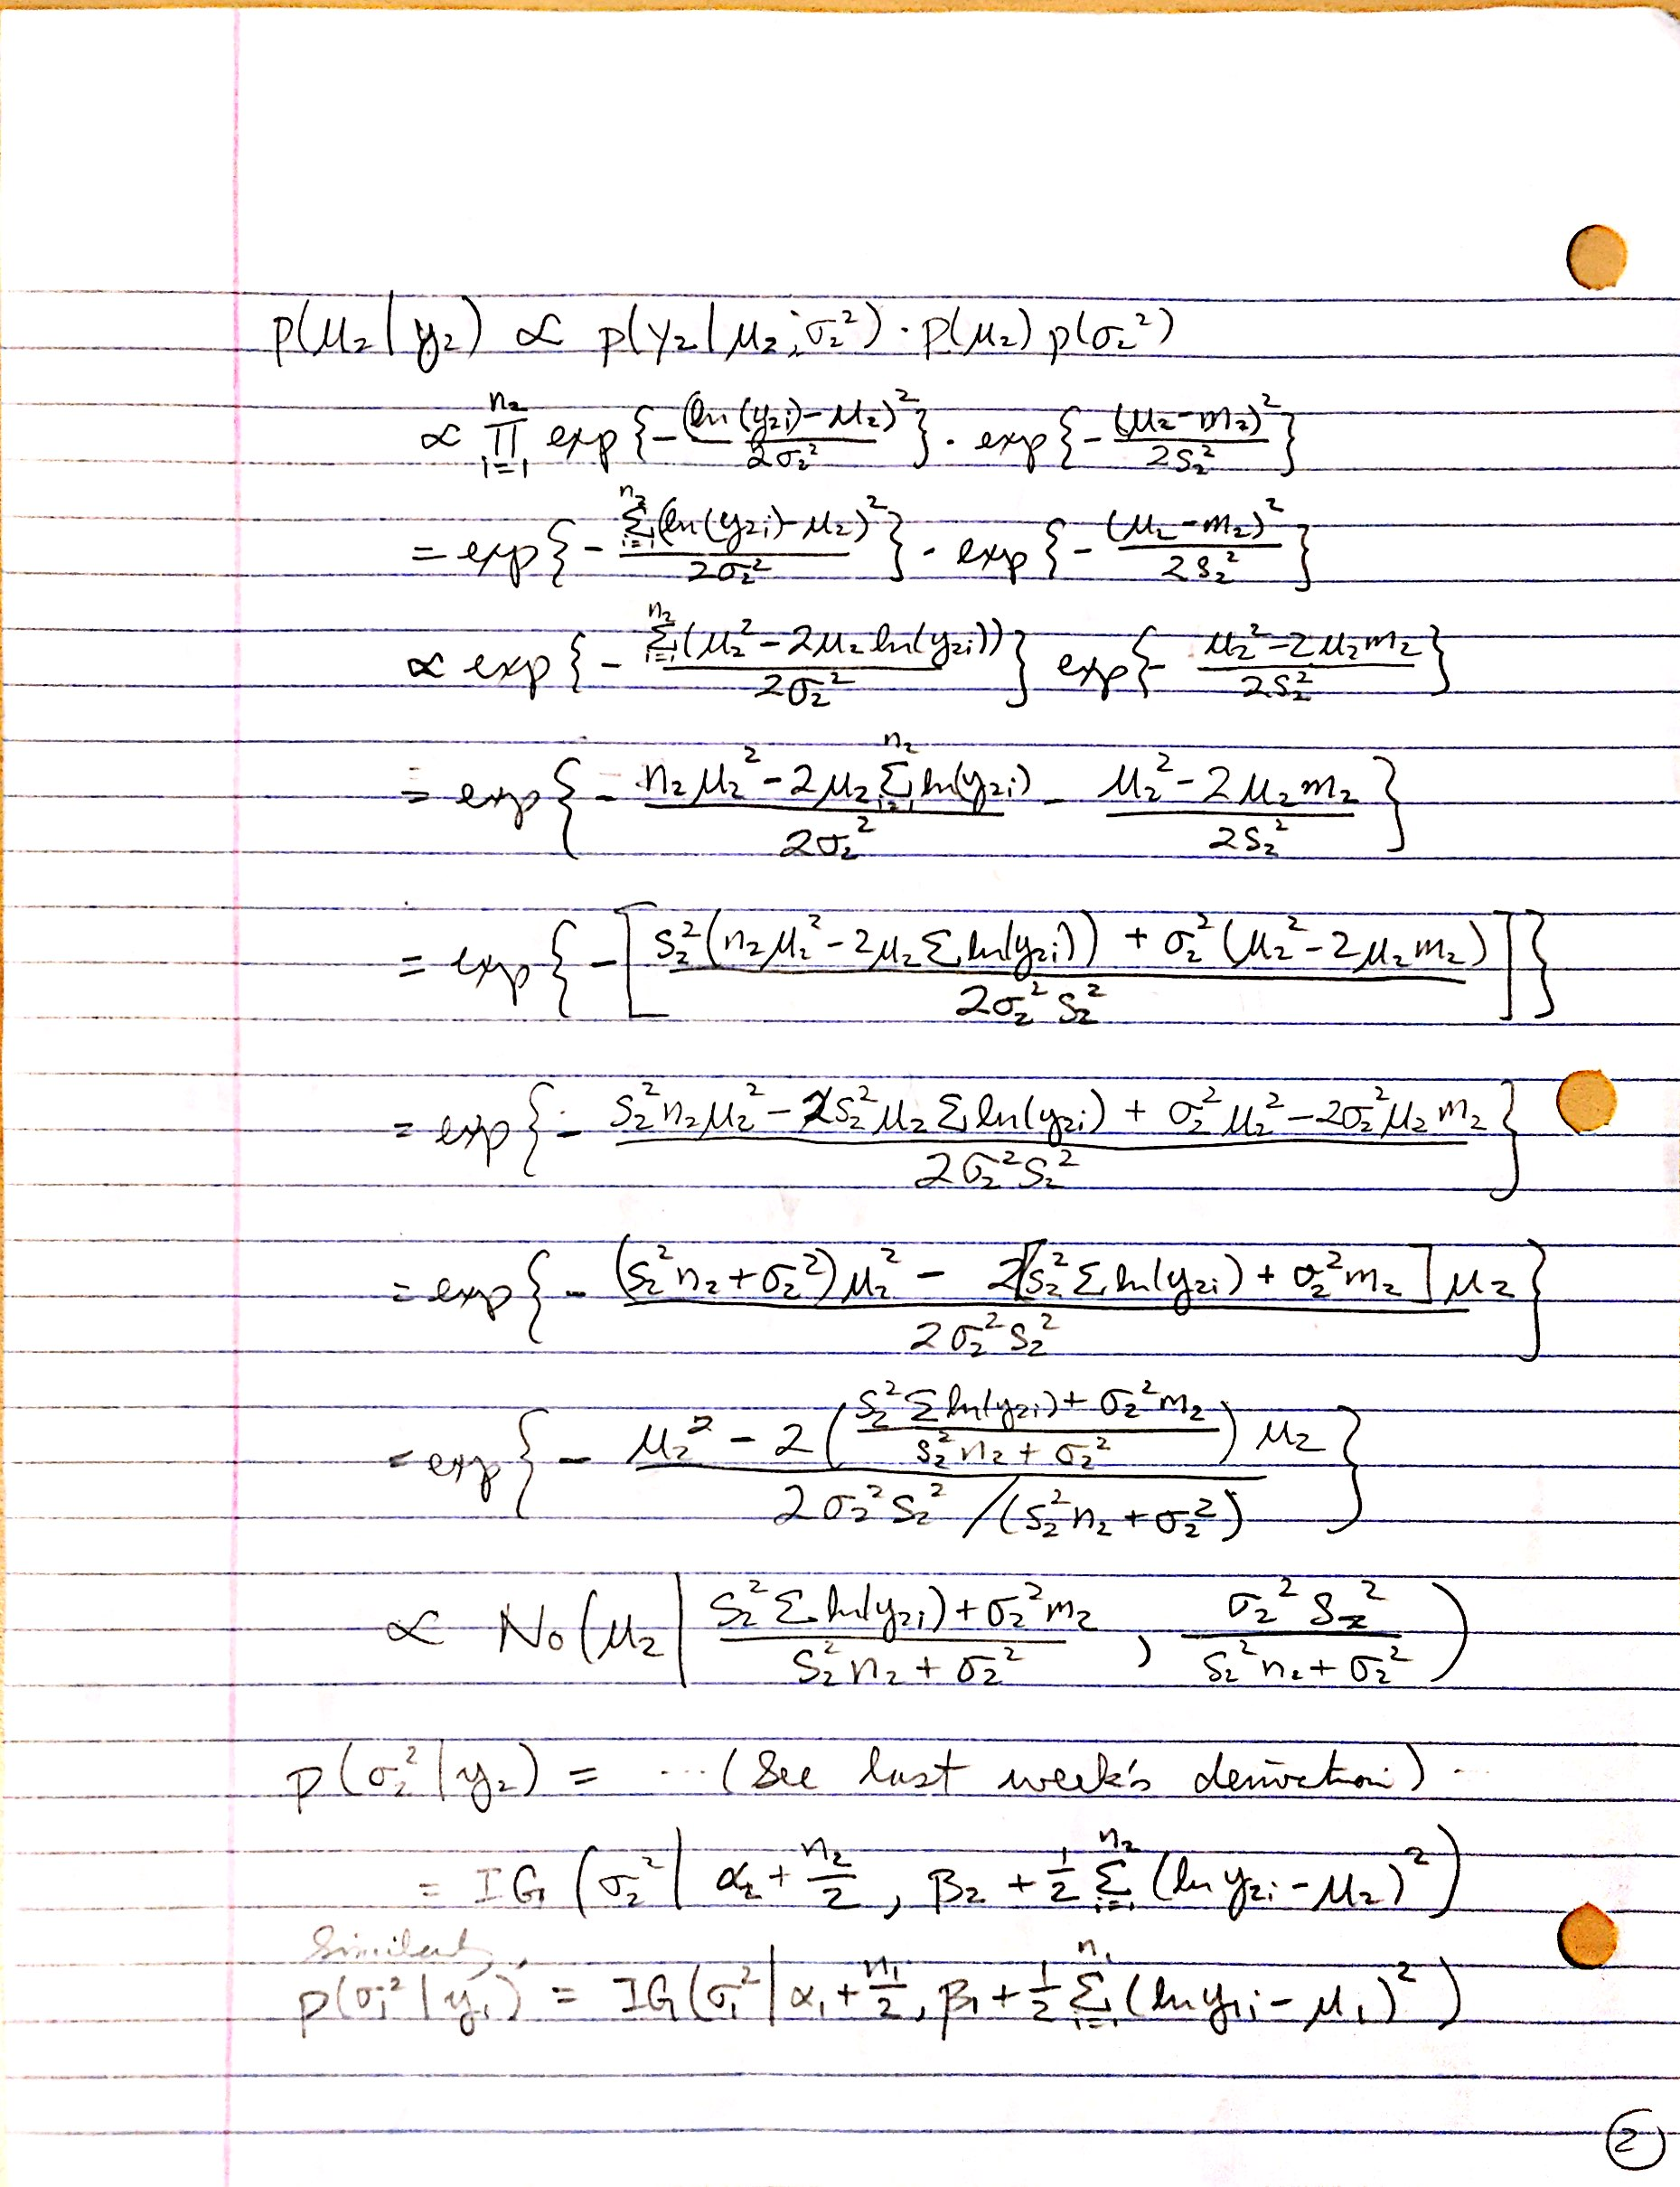
\includegraphics[scale=0.23]{page2.jpg} \\
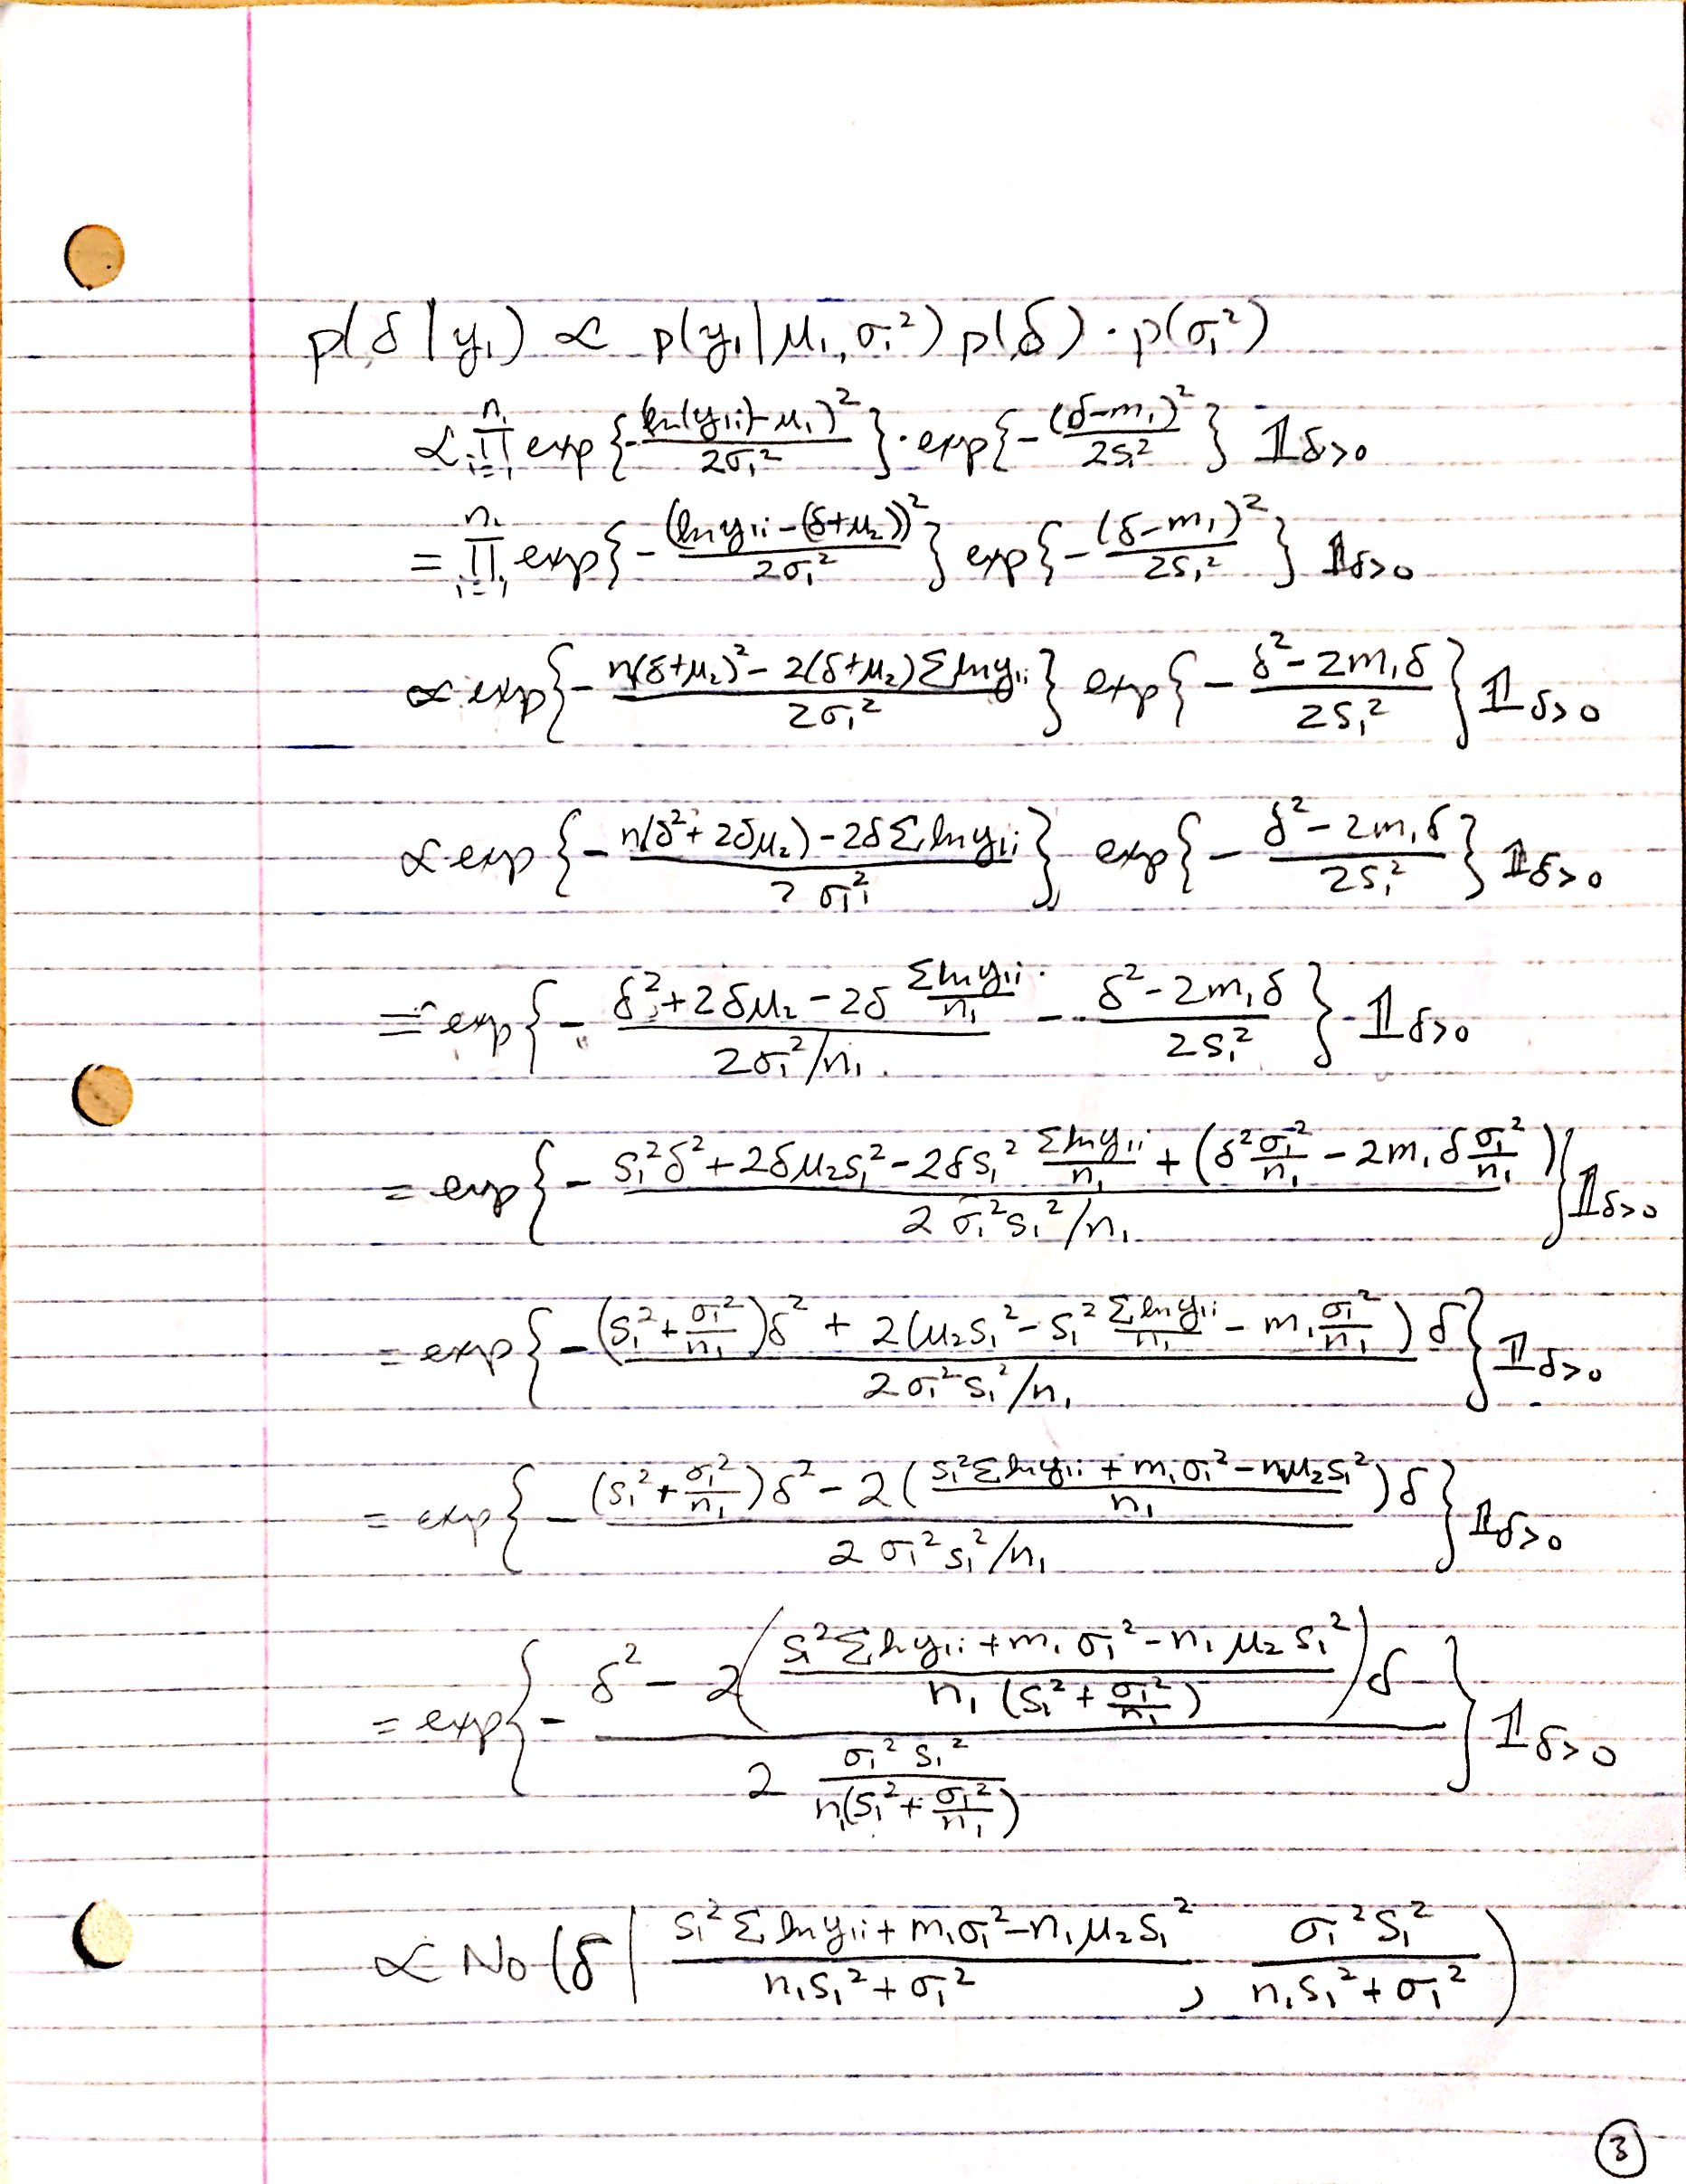
\includegraphics[scale=0.23]{page3.jpg}

\pagebreak

\item Below are traceplots of $\mu_1 $ and $\sigma_1^2$:

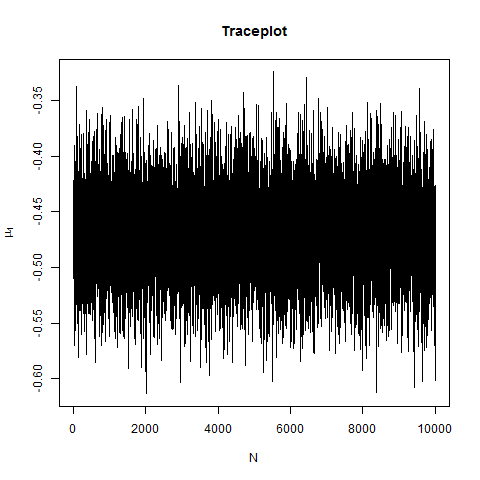
\includegraphics[scale = 0.4]{MU1plot.png}
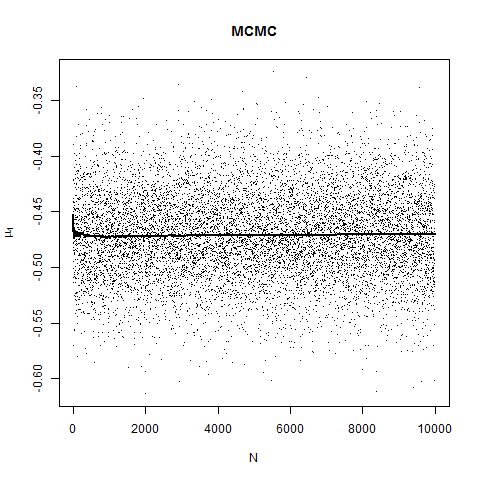
\includegraphics[scale = 0.4]{MU1MCMC.png}\\
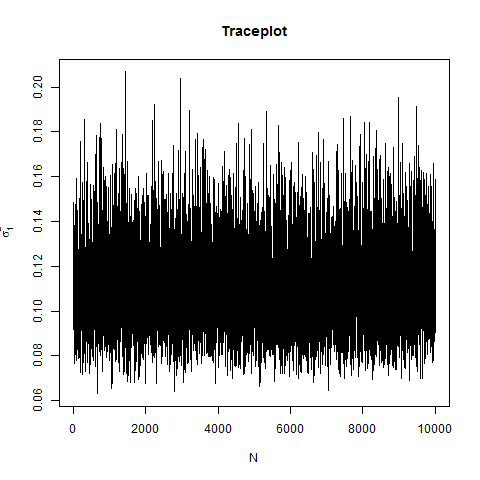
\includegraphics[scale = 0.4]{SIG1plot.png}
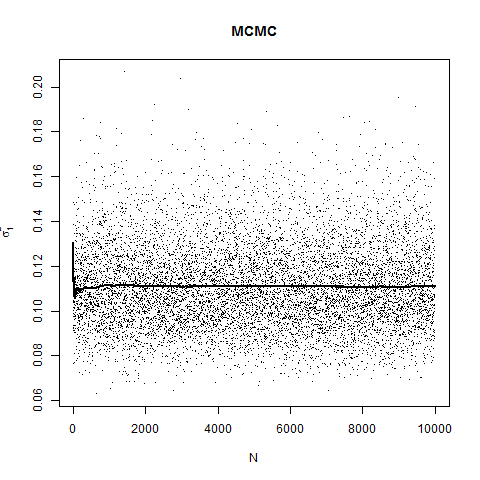
\includegraphics[scale = 0.4]{SIG1MCMC.png}\\

\item Below are point estimates and 95\% confidence intervals:
\begin{center}
\begin{tabular}{r||c|c}
& Mean & Confidence Interval \\ \hline
$\mu_1$ & -0.4708718 & [-0.5466545, -0.3949325] \\ \hline
$\mu_2$ & -1.377839 & [-1.5240060, -1.2294750] \\ \hline
$\sigma_1^2$ & 0.1104881 & [0.07978934, 0.15334020] \\ \hline
$\sigma_2^2$ & 0.1597617 & [0.09405123, 0.26961285]
\end{tabular}

\end{center}

\item Posterior probability that $\mu_1>\mu_2$ is 1. Posterior probability that $\sigma_1^2 > \sigma_2^2$ is 0.136.

\item The posterior probability that the pollution level on a randomly chosen future Tuesday is higher than the pollution level on a randomly chosen future Saturday is 0.9579.


\end{enumerate}

\pagebreak

See below for R code:
\listinginput[1]{1}{lab10.r}

\end{document}